\documentclass[conference]{IEEEtran}

\usepackage{amsmath}
\usepackage{amssymb}
\usepackage{booktabs}
\usepackage{array}
\usepackage{graphicx}
\usepackage{multirow}
\usepackage{url}
\usepackage{cite}
\usepackage{xcolor}
\usepackage{xspace}
\usepackage[hidelinks]{hyperref}
\usepackage{tabularx}
\usepackage{threeparttable}

\newcommand{\code}[1]{\texttt{#1}}

\def\BibTeX{{\rm B\kern-.05em{\sc i\kern-.025em b}\kern-.08em
    T\kern-.1667em\lower.7ex\hbox{E}\kern-.125emX}}

% Global float padding reduction
\setlength{\textfloatsep}{6pt plus 1.0pt minus 2.0pt}
\setlength{\floatsep}{6pt plus 1.0pt minus 2.0pt}
\setlength{\intextsep}{6pt plus 1.0pt minus 2.0pt}

\begin{document}

\title{Pre-Authorization Screening of EIP-7702 Delegates\\under an Adaptive Adversary}

\maketitle

\begin{abstract}
EIP-7702 lets an Ethereum externally owned account delegate code execution to a smart contract, creating a security decision at authorization time when behavioral history, reputation, and verified source code may all be unavailable while the delegate's runtime bytecode is already observable. We study whether that bytecode alone supports pre-authorization risk screening, and we argue that the usual measure of such a screener---clean classification accuracy---does not answer the question that matters. On an audited, family-disjoint benchmark of 2,190 observed delegates in 790 bytecode-similarity families, four very different screeners reach comparable clean performance, including a 15-feature logistic regression that is statistically indistinguishable from our neural model. Under a query-budgeted adaptive adversary restricted to structurally valid, bounded-overhead bytecode edits, they separate sharply: attack success rises to 0.986 for a histogram gradient-boosting model and 0.945 for a flat convolutional encoder, while our hierarchical chunk-attention model, AuthGuard-Seq, holds at 0.181. Crucially, a fixed-transformation study---the standard protocol in prior bytecode security learning---cannot distinguish AuthGuard-Seq from the cheap emulator at all ($+0.082$, 95\% CI $[-0.047,+0.218]$); only adaptive search resolves them ($+0.360$, CI $[+0.188,+0.518]$). Parameter-matched ablations attribute the difference to length-invariant attention aggregation rather than to sequence coverage or hierarchy as such. We further report the first operational measurement of such a screener on live delegation traffic---752 Ethereum delegates observed over a two-week window disjoint from the benchmark at the bytecode-family level---and a measured 652$\times$ cost gap against a reference decompiler that motivates millisecond screening ahead of selective deep analysis.
\end{abstract}

\begin{IEEEkeywords}
EIP-7702, Ethereum, smart contract security, bytecode analysis, adversarial robustness, trust in delegated execution, security evaluation methodology
\end{IEEEkeywords}

\section{Introduction}
\label{sec:intro}

Ethereum traditionally separates externally owned accounts (EOAs), controlled by user keys, from smart contracts that carry executable logic. EIP-7702 changes this by letting an EOA delegate code execution while keeping its address~\cite{eip7702}. This enables transaction batching, gas sponsorship, and programmable authorization, but it also moves execution authority over an account's assets, approvals, and transaction behavior to third-party code. Authorizing an unsafe delegate is therefore a trust decision made under information scarcity: a newly deployed delegate may have no transaction history, no reputation, and no verified source, yet its runtime bytecode can already be fetched from chain. Figure~\ref{fig:riskwindow} shows this window.

This paper asks whether bytecode alone supports screening at that boundary, and how such a screener should be evaluated. Our central claim is that the second question determines the answer to the first. Pre-authorization screening is an adversarial setting by construction: the attacker writes the bytecode being screened and can pad, reorder, or rewrite it for little more than deployment gas. A screener that is accurate on unmodified code but collapses under cheap edits provides no protection against the adversary it exists to stop.

We find this distinction is not hypothetical. Four screeners spanning gradient boosting, flat convolution, hand-engineered control-flow features, and hierarchical attention reach broadly similar clean performance on our benchmark, and a 15-feature logistic regression is statistically indistinguishable from our neural model ($\Delta$AUPRC $-0.021$, 95\% CI $[-0.078,+0.035]$). Under a query-budgeted adaptive attacker they separate by a factor of five. More pointedly, the protocol used throughout prior bytecode security learning---evaluating on one fixed transformation---cannot separate our model from the cheap emulator at all, while adaptive search separates them decisively. The evaluation instrument, not the model, is what resolves the question.

\begin{figure}[t]
\centering
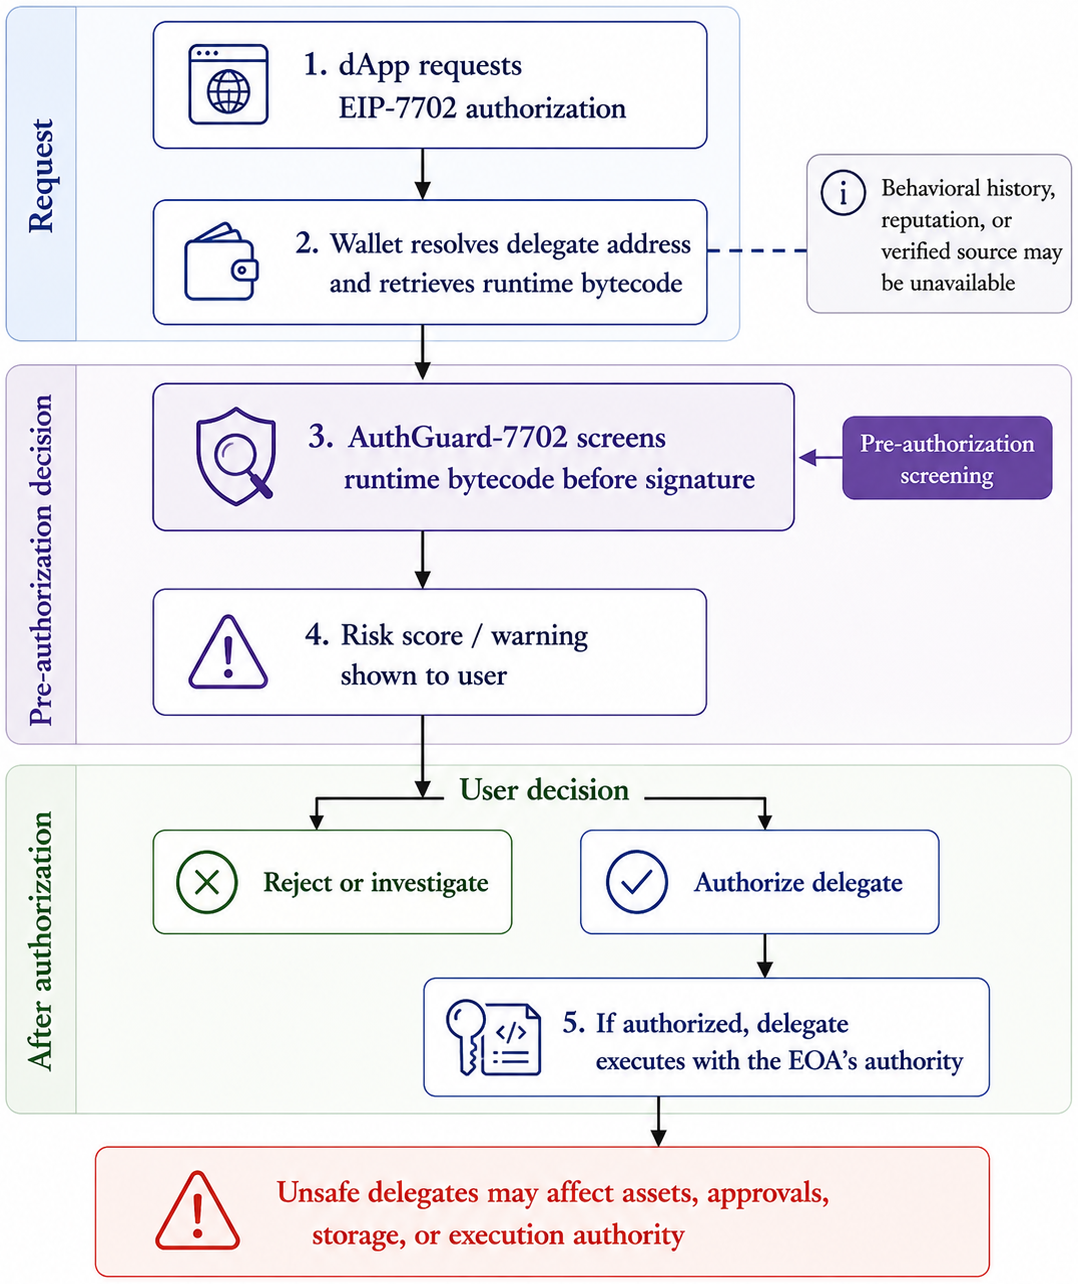
\includegraphics[width=\columnwidth]{eip_7702_authorization_risk_flowchart.png}
\caption{EIP-7702 authorization flow and the pre-signature screening window.}
\label{fig:riskwindow}
\end{figure}

We present AuthGuard-7702, a bytecode-only screening framework producing a calibrated score and warning tier, built around AuthGuard-Seq: a compact hierarchical model that disassembles runtime bytecode, splits the opcode stream into 256-token chunks, encodes local order with shared convolutions, and aggregates chunk evidence with learned attention. It uses 63{,}266 active parameters, processes up to 16{,}384 opcodes, and consumes no transaction history, source code, address identity, or reputation metadata.

A second concern is dependence among contract samples. Code duplication inflates measured performance of learned models of code~\cite{allamanis2019duplication}, and contract corpora contain redeployments and near-duplicate variants that let row-level random splits place related programs on both sides of a split~\cite{tesseract2019}. We audit the source data, build bytecode-similarity families, keep identical and related bytecode within one fold, and exclude observations with unreliable source verdicts.

The study makes three contributions.

\begin{itemize}
    \item \textbf{An adversarial evaluation methodology for bytecode security classifiers, and the design finding it yields.} We contribute a query-budgeted adaptive attack over a defined bytecode action space with bounded byte overhead, per-candidate structural validity checking, and a bounded execution-preservation audit, applied across four architecture families with cross-model transfer. It shows that fixed-transformation evaluation is insufficient to rank screeners, and parameter-matched ablations attribute robustness specifically to length-invariant attention aggregation.
    \item \textbf{An audited benchmark with a live temporal holdout.} AuthGuardBench-7702 combines 2,190 audited delegates in 790 families under family-disjoint cross-validation with external benign controls, an audited-implementation registry, and 752 independently collected live Ethereum delegates from a strictly later two-week window, disjoint at the family level.
    \item \textbf{Operational evidence for staged triage.} We measure the complete local screening path at 4.121\,ms median against a pinned reference decompiler at 2.687\,s median---a 652$\times$ gap---and report flag rates on live delegation traffic weighted by observed authorization volume.
\end{itemize}

We do not claim architectural novelty. Every component of AuthGuard-Seq is standard; the contribution is the adversarial requirement that motivates the design, the evaluation that isolates which mechanism satisfies it, and the honest negative controls that bound what the model adds.

\section{Background and Related Work}
\label{sec:related}

\subsection{EIP-7702 and the Authorization Boundary}

EIP-7702 introduces authorization tuples through which an EOA delegates code execution while keeping its address. For each valid tuple a delegation indicator formatted as $\code{0xef0100}\Vert\code{address}$ is written to the authorizing EOA's code field, and subsequent code-executing operations resolve and run the code at the referenced delegate~\cite{eip7702}. The object worth screening is therefore the delegate's runtime bytecode, not the 23-byte indicator. Once authorized, that code executes in the EOA's context, which makes the pre-signature moment the natural automation point.

Huang et al. combine transaction analysis with cross-contract static analysis to characterize EIP-7702 malicious behavior~\cite{huang2026darkside}; Qi et al. study delegation-based phishing and protocol defenses~\cite{qi2025eip7702}. Neither investigates learned screening of proposed delegate bytecode before authorization.

\subsection{Learning from Smart-Contract Bytecode}

ContractWard uses opcode bigrams with conventional learners~\cite{contractward2021}, Eth2Vec learns contract-wide bytecode representations~\cite{eth2vec2022}, PhishingHook evaluates bytecode and opcode representations for phishing-contract classification~\cite{phishinghook2025}, and more recent work combines bytecode features with control-flow-graph analysis~\cite{smartbugbert2025}. Surveys identify representation, dataset construction, and evaluation design as recurring determinants of reported performance~\cite{wang2026review}.

These works share an evaluation posture: they report clean classification metrics and do not evaluate an adversary who controls the input program. That is the gap this paper addresses. Since the attacker authors the bytecode, clean metrics measure the easy case. Table~\ref{tab:related} summarizes the positioning.

\begin{table}[t]
\centering
\caption{Comparison with representative prior work}
\label{tab:related}
\begin{threeparttable}
\scriptsize
\begin{tabularx}{\columnwidth}{@{}X c c c c@{}}
\toprule
Work & EIP-7702 & Bytecode ML & Pre-auth. & Adaptive adv. \\
\midrule
Huang et al.~\cite{huang2026darkside} & \checkmark & -- & -- & -- \\
Qi et al.~\cite{qi2025eip7702} & \checkmark & -- & -- & -- \\
PhishingHook~\cite{phishinghook2025} & -- & \checkmark & -- & -- \\
Eth2Vec~\cite{eth2vec2022} & -- & \checkmark & -- & -- \\
ContractWard~\cite{contractward2021} & -- & \checkmark & -- & -- \\
SmartBugBert~\cite{smartbugbert2025} & -- & \checkmark & -- & -- \\
\textbf{AuthGuard-7702} & \checkmark & \checkmark & \checkmark & \checkmark \\
\bottomrule
\end{tabularx}
\begin{tablenotes}[flushleft]
\scriptsize
\item[] ``Adaptive adv.'' denotes evaluation against an attacker who searches over input modifications with knowledge of the screener's scores, as opposed to a fixed predefined transformation.
\end{tablenotes}
\end{threeparttable}
\end{table}

\subsection{Static Analysis and Security-ML Evaluation}

Learned screening complements rather than replaces semantic analysis. Gigahorse decompiles EVM bytecode for declarative analysis~\cite{gigahorse2019} and Securify derives semantic dependencies and checks security patterns~\cite{securify2018}. Our reference labels originate from a decompiler-based rule~\cite{huang2026darkside}; our question is whether that signal can be approximated from opcode sequences fast enough for interactive screening, and whether such an approximation survives an adversary.

Methodology matters as much as modeling. TESSERACT shows how dependence and distribution bias inflate security-classification results~\cite{tesseract2019}. We isolate identical and similar bytecode families across folds, and we interpret transformed executable inputs only within their demonstrated preservation guarantees, following problem-space adversarial-ML guidance~\cite{pierazzi2020}.

\begin{figure*}[t]
\centering
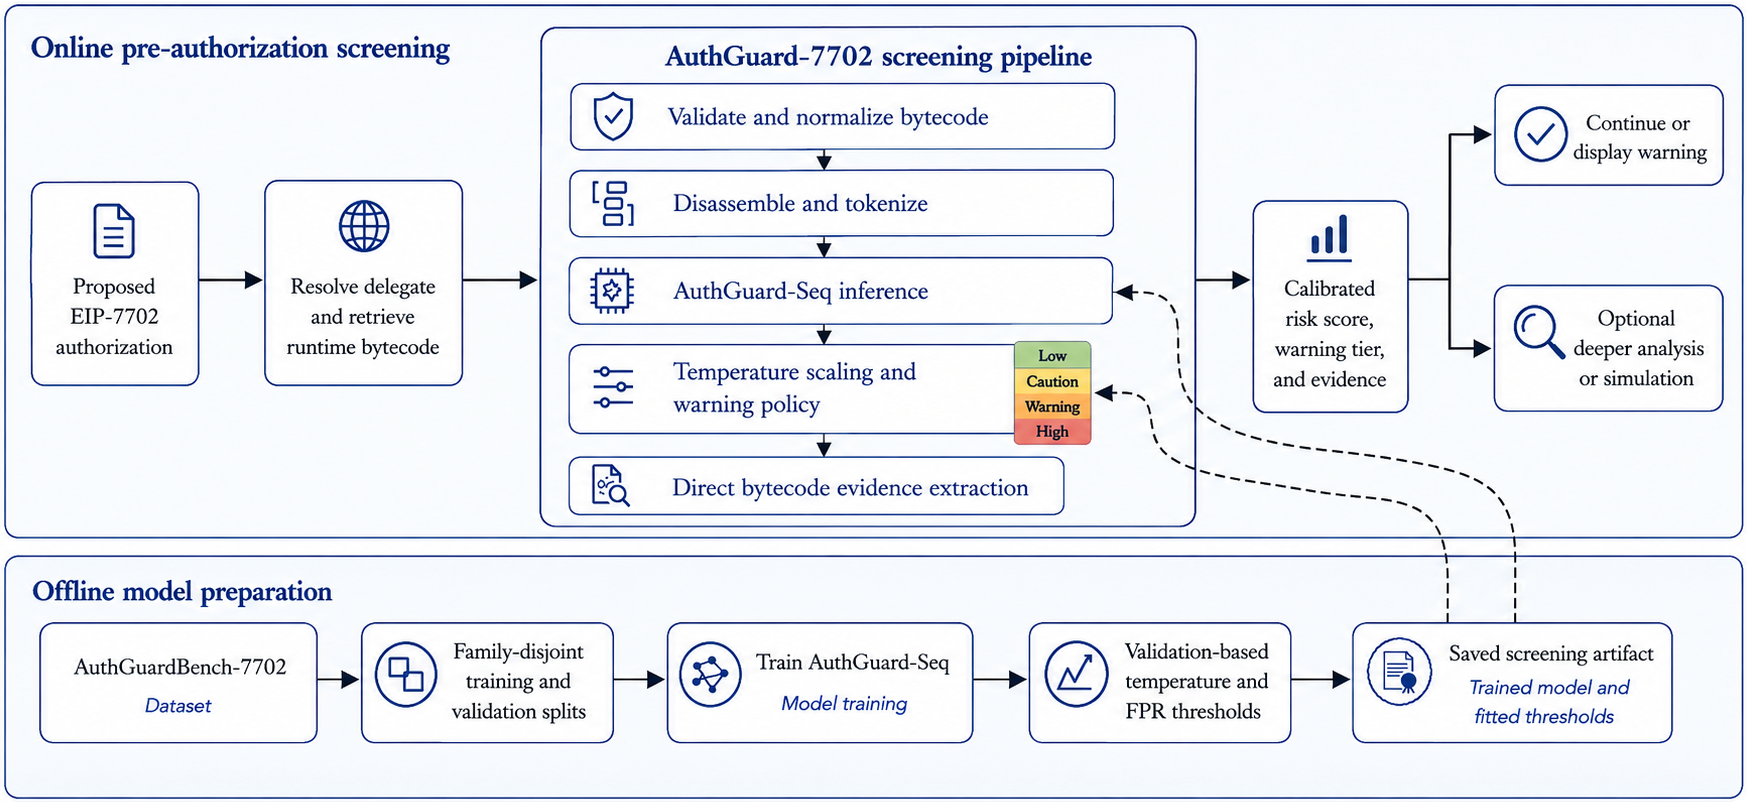
\includegraphics[width=0.98\textwidth]{figure-1-bak.png}
\caption{AuthGuard-7702 system overview: the online screening path at the authorization boundary and the offline family-disjoint training and calibration path.}
\label{fig:decision}
\end{figure*}

\section{Problem Formulation and Threat Model}
\label{sec:problem}

\subsection{Pre-Authorization Screening Task}

Let $b$ be the normalized runtime bytecode at a proposed delegate address and $T(b)$ its opcode-token sequence. A trained model $f_\theta$ produces a risk logit that is temperature-scaled on validation data~\cite{guo2017calibration}:

\begin{equation}
s(b)=\sigma\!\left(\frac{f_\theta(T(b))}{T_{\mathrm{cal}}}\right),
\qquad
T_{\mathrm{cal}}>0,
\qquad
s(b)\in[0,1].
\label{eq:score}
\end{equation}

The positive class consists of delegates flagged by the source study's static-analysis rule, which identifies decompiled reachability from standardized inbound hooks---\code{receive()}, \code{fallback()}, and token-reception callbacks---to predefined value-moving external-call patterns~\cite{huang2026darkside}. The negative class is delegates from the same pool that were not flagged. Because an unflagged verdict does not establish benign semantics, the task is screening for source-analyzer-identified structural risk, not proving malicious intent, exploitability, or safety. We use ``source-flagged'' rather than ``malicious'' throughout.

This label provenance is a real limitation, and we address it in two ways rather than one. First, we scope every claim to the reference condition. Second, and more importantly, our headline result is a \emph{relative} comparison among architectures evaluated against a shared label under a shared adversary. Whatever the label denotes, the ranking of screeners under attack is a statement about the screeners, and does not require the label to be adjudicated ground truth. This is the principal reason we organize the paper around adversarial robustness rather than absolute detection quality.

From negative validation scores we derive thresholds $\tau_1\geq\tau_5\geq\tau_{10}$ for nominal 1\%, 5\%, and 10\% false-positive-rate (FPR) operating points, mapping scores to \textsc{High}, \textsc{Warning}, \textsc{Caution}, and \textsc{Low-Observed-Risk}. Because thresholds are estimated on finite validation sets, realized FPR can differ from nominal, and Section~\ref{sec:rq3} measures how far.

\subsection{Information Boundary}

The model observes only the ordered opcode sequence derived from runtime bytecode. PUSH immediate operands are skipped, so the representation captures opcode identity and order rather than embedded constants. The model receives no transaction history, balances, approvals, graph or address identity, source code, family or fold identifiers, or any field used to construct the reference labels. This boundary is deliberate: the intended case is a delegate with no historical or identity evidence. AuthGuard-7702 is an advisory first-stage screener; it does not resolve proxy state, simulate transactions, infer off-chain intent, or certify safety.

\subsection{Adversary Model}

We consider an adversary who wants a delegate whose runtime code exhibits the reference risk condition to be authorized, and who therefore wants that code to score below the wallet's warning threshold. The adversary \textbf{authors the bytecode}. We grant them:

\begin{itemize}
\item \emph{Score access.} They may query the screener and observe its output, as they can for any locally deployed or publicly reachable model. We bound this at 64 queries per contract.
\item \emph{Edit capability.} They may append content, rewrite metadata, and rewrite embedded address and selector immediates, composing up to four such actions.
\item \emph{A cost budget.} Edits are capped at $2\times$ the original executable size, since deployment cost scales with code size.
\end{itemize}

We do \emph{not} grant white-box gradient access or the ability to retrain the defender's model. The defender is a wallet or security service that fetches the proposed delegate's runtime bytecode and applies AuthGuard-7702 before authorization; we assume correct retrieval and trusted model parameters. Compromise of the wallet, signing key, retrieval infrastructure, or screener is out of scope.

The model can only detect risk observable from runtime bytecode. Behavior depending on dynamic state, transaction context, unresolved proxy targets, external counterparties, or off-chain intent may remain invisible.

\section{AuthGuard-7702}
\label{sec:system}

\subsection{Screening Workflow}

Figure~\ref{fig:decision} places AuthGuard-7702 at the authorization boundary. A wallet resolves the proposed delegate address, retrieves runtime bytecode, and invokes the local path before the user signs. The pipeline normalizes and disassembles the bytecode, runs AuthGuard-Seq, applies validation-fitted calibration and thresholds, and returns a score, warning tier, and auxiliary bytecode evidence. Offline, the training path constructs family-disjoint folds, trains the model, and fits the temperature and FPR thresholds on validation data only; the resulting artifact is what the online path loads.

Auxiliary evidence is extracted separately from raw bytecode and includes code length, opcode counts, call-family instructions, storage writes, contract-creation instructions, and recognized token-transfer or approval selectors. These observations and the learned attention weights indicate influential regions; they are not causal explanations or control-flow proofs.

\subsection{Design Under an Adversarial Requirement}

The design follows from the adversary model rather than from architectural ambition. Because the attacker controls program length and can append arbitrary content cheaply, the aggregation step must not let appended bytes dilute or dominate the risk signal. This yields three requirements, each tied to an attack and each tested in Section~\ref{sec:rq1}:

\begin{enumerate}
\item \emph{Full-stream coverage.} Fixed-window models can be evaded by pushing the payload past the window, so the model must see the whole program rather than a prefix.
\item \emph{Local order sensitivity.} Histogram and $n$-gram representations discard instruction order, which order-preserving rewrites exploit; local convolutions retain short ordered motifs.
\item \emph{Length-invariant, selective aggregation.} Mean pooling over a longer program dilutes evidence proportionally to appended content. Learned attention can concentrate on the informative region regardless of how much padding surrounds it.
\end{enumerate}

\subsection{Hierarchical Opcode-Sequence Model}

AuthGuard-Seq begins with deterministic linear-sweep EVM disassembly. Recognized opcodes map to stable token IDs, undefined bytes use a dedicated token, and padding uses a separate ID. PUSH immediates are skipped by instruction width. Tokenization does not terminate at the first linear \code{STOP}, so trailing regions are not discarded because of an early stopping opcode. The sequence is split into chunks of length $L=256$, at most $K=64$ chunks. The longest benchmark program has 16{,}081 opcodes and fits the 16{,}384-token capacity, so every benchmark contract is processed in full; longer contracts outside the benchmark retain evenly spaced chunks rather than a prefix.

Each chunk is embedded into 32 dimensions, processed by a kernel-5 convolution followed by a kernel-3 dilated convolution with dilation 2, and reduced by masked maximum pooling to a 64-dimensional $h_k$. Learned attention aggregates valid chunks:

\begin{equation}
\alpha_k=\frac{\exp(w^\top h_k)}{\sum_{j=1}^{K_b}\exp(w^\top h_j)},
\qquad
h=\sum_{k=1}^{K_b}\alpha_k h_k,
\label{eq:attention}
\end{equation}

where $w$ is learned and $K_b$ is the number of non-padding chunks. The aggregate passes through a 128-dimensional layer with GELU, dropout, layer normalization, and a binary risk head. The logit is temperature-scaled before thresholds apply. Figure~\ref{fig:encoder} summarizes the architecture.

\begin{figure*}[t]
\centering
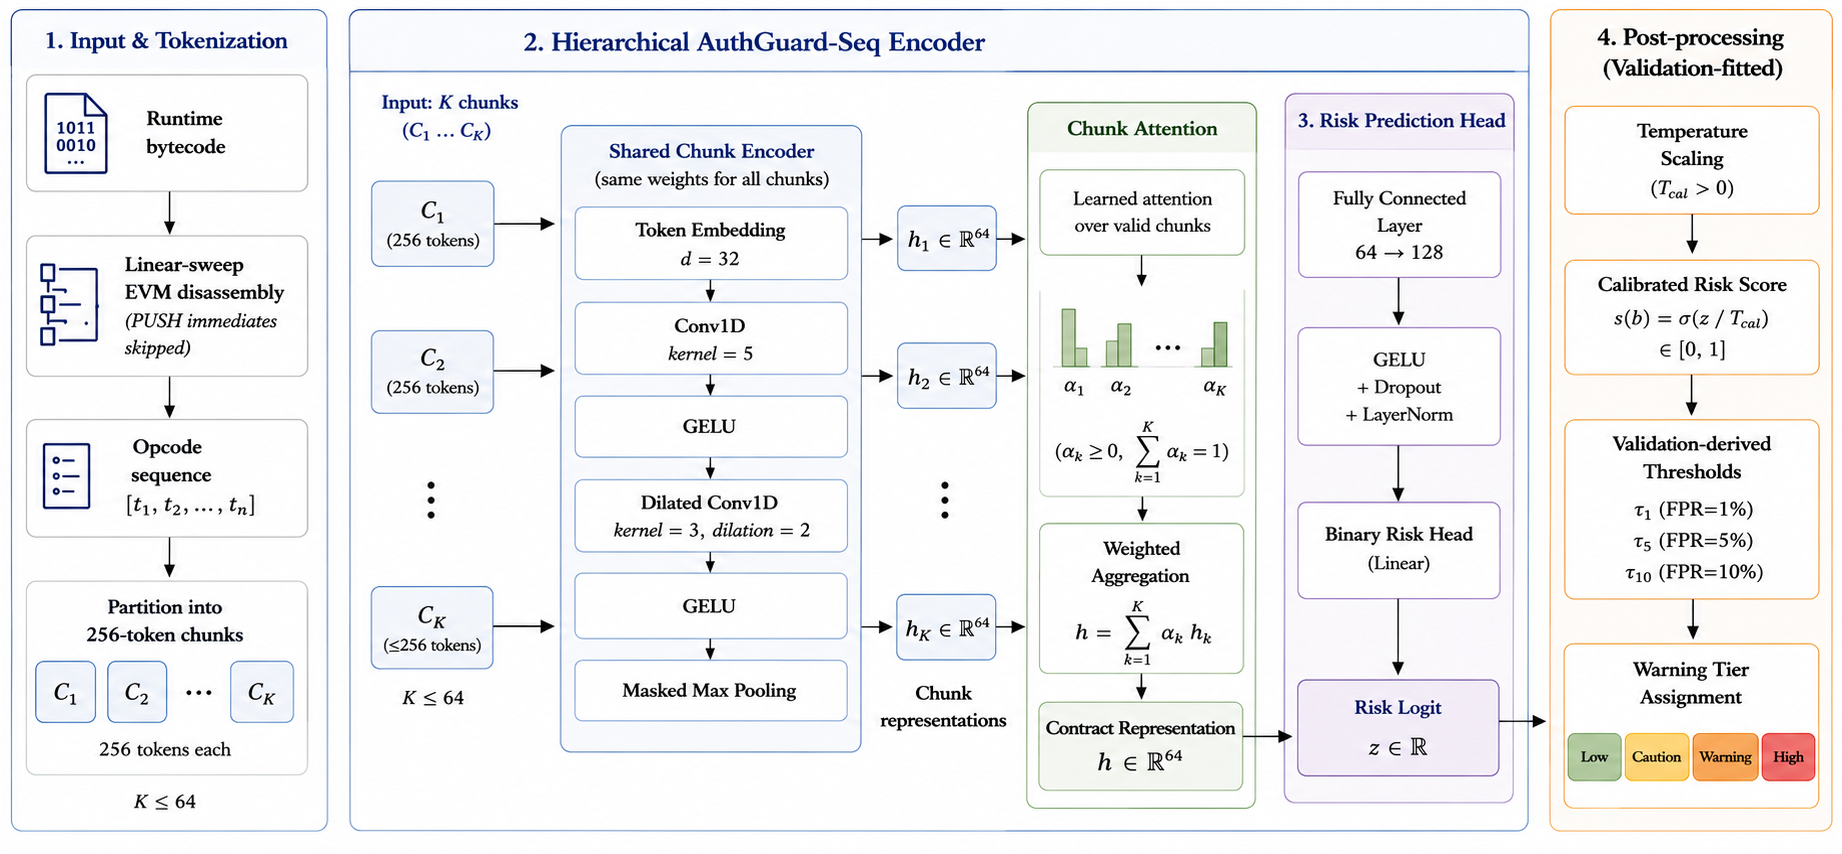
\includegraphics[width=0.98\textwidth]{figure-2-fixed.png}
\caption{AuthGuard-Seq: chunked opcode encoding, shared local convolutional encoders, and learned chunk attention. Attention aggregation is the mechanism the ablation in Table~\ref{tab:ablation} isolates as responsible for robustness under bytecode flooding.}
\label{fig:encoder}
\end{figure*}

\paragraph*{Parameter accounting} AuthGuard-Seq is the sequence-only configuration of a fusion architecture that also defines $n$-gram and dense-structural branches. Those branches are constructed but receive no gradient in this configuration, so a naive parameter sum over the module overstates the model and, worse, reports an identical count for configurations that differ. We report parameters that are actually on the trained forward path, verified by checking which tensors receive gradient: \textbf{63{,}266} for AuthGuard-Seq, against 108{,}225 for the $n$-gram variant and 75{,}595 for the dense-structural variant. The serialized checkpoint used for timing is 742{,}625\,bytes because it stores all constructed branches.

\section{Benchmark and Methodology}
\label{sec:method}

\subsection{Audited Benchmark Construction}

\textit{AuthGuardBench-7702} contains 3,082 audited observations partitioned before evaluation (Table~\ref{tab:dataset}). The primary population derives from the EIP-7702 delegate dataset and analyzer outputs of Huang et al.~\cite{huang2026darkside}; after auditing it holds 2,190 delegates, 727 source-flagged and 1,463 unflagged. External controls contribute 797 benign-labeled general Ethereum contracts from the PhishingHook-derived source~\cite{phishinghook2025}, and eight audited production EIP-7702 implementations provide named qualitative controls. A further 90 observations are excluded because their original unflagged verdicts came from truncated or failed bytecode retrieval: we identified 89 negatives truncated at a spreadsheet cell limit and one timeout string stored in place of bytecode. Although the runtimes were recoverable, the verdicts had not been established on repaired inputs.

Section~\ref{sec:rq3} adds a fourth population collected independently for this work: 752 screenable Ethereum delegates observed in a two-week window strictly later than the benchmark.

\begin{table}[t]
\centering
\caption{Audited benchmark populations}
\label{tab:dataset}
\scriptsize
\begin{tabularx}{\columnwidth}{@{}X r X r@{}}
\toprule
Population & $n$ & Reference status & Families \\
\midrule
Primary evaluation & 2,190 & 727 flagged / 1,463 unflagged & 790 \\
External benign control & 797 & Benign-labeled & -- \\
Audited implementations & 8 & Named production delegates & -- \\
Excluded uncertain input & 90 & Unreliable source verdict & -- \\
\midrule
Live temporal holdout & 752 & Unlabeled & 454 \\
\bottomrule
\end{tabularx}
\end{table}

\subsection{Families, Duplicates, and Splits}

Runtime bytecode is linearly disassembled and represented as opcode 4-gram sets. Deterministic 128-permutation BLAKE2b MinHash signatures with a fixed 0.85 agreement threshold define similarity links, merged by union-find into 790 families. Identical bytecode with conflicting reference labels is quarantined before modeling.

We use five fixed family-disjoint outer folds. For test fold $f$, fold $(f+1)\bmod 5$ is validation and the remaining three are training. No family or identical bytecode crosses folds. Each configuration is repeated with seeds 7702, 7703, and 7704; results average five folds within a seed and then report mean and sample standard deviation across the three seed-level means.

\subsection{Adaptive Attack Protocol}
\label{sec:attackproto}

The attack searches over compositions of eight actions: metadata rewrite; embedded address rewrite; function-selector rewrite; neutral instruction insertion; and flooding that appends a \code{STOP} followed by deterministic donor bytes at 25\%, 50\%, 100\%, or 200\% of the source executable length. At most one flooding action and at most four actions total may compose.

Two search strategies share a 64-query budget per contract: a seeded \emph{random search} over sampled action sequences, and a score-guided \emph{beam search} with width 4 and depth 4 that expands the lowest-scoring candidates. Both are deterministic given the seed. We additionally evaluate each fixed transformation alone and a per-source oracle over the seven fixed conditions.

Three constraints keep the attack honest. Every candidate must be \textbf{structurally valid}, i.e. disassemble and satisfy an opcode-skeleton preservation check against the source. Every candidate must respect a \textbf{$2\times$ byte-overhead cap}. Flooding donors are drawn from partition-isolated pools such that a donor never shares the recipient's bytecode family and never crosses the train/validation/test boundary, with full provenance recorded per segment.

An attack \emph{succeeds} on a source if the clean score is at or above the model's own validation-derived 5\% FPR threshold and the adversarial score falls below it. Attack success rate (ASR) is computed over sources the model detects cleanly, since a source it never flagged cannot be evaded. Each architecture is attacked as the target in turn, and each target's best candidate is scored by the other models to give transfer rates.

\paragraph*{Execution preservation} A bounded audit of 100 calls across ten delegates compares source and transformed execution. Flooding preserved recorded execution behavior in 100/100 calls. Address-immediate rewriting preserved only 23/100, so conditions involving it are reported as representation stress, not behavior-preserving, and we mark them accordingly. We claim bounded empirical preservation for flooding, not universal semantic equivalence.

\subsection{Baselines, Training, and Statistics}

The clean comparison evaluates seven predefined configurations under identical folds, validation rotation, seeds, early stopping, calibration, and operating points. Nonhierarchical neural baselines use a 2,048-position opcode view obtained by uniform sampling across the whole stream; AuthGuard-Seq processes complete streams in at most 64 chunks of 256 tokens. Neural models use class-weighted binary cross-entropy with positive-class weight equal to the training-fold negative-to-positive ratio, AdamW at learning rate $10^{-3}$, weight decay $10^{-4}$, gradient clipping at 5, at most 30 epochs, and validation-AUPRC early stopping with patience 5. Temperature scaling is fit on validation logits only and thresholds derive only from negative validation examples. Test labels never influence model selection, calibration, or thresholds.

AUPRC is the primary ranking metric because the population is imbalanced and the metric emphasizes positive-class ranking; AUROC and calibrated Brier score are secondary. Operational behavior is Recall@5\% FPR. For inferential comparisons the bytecode family is the resampling unit: families are resampled with replacement within each outer test fold and the same multiplicities apply to both members of a pair. \textbf{Replicate counts differ by experiment and we state them per table}: 10{,}000 for primary clean comparisons, 2{,}000 for the mechanism ablation, and 1{,}998 for the cheap-baseline controls.

\section{Evaluation}
\label{sec:evaluation}

We ask four questions. RQ1: what does clean screening actually require, and which mechanism supplies it? RQ2: which screeners survive an adversary who writes the bytecode? RQ3: do calibrated operating points transfer across time and population? RQ4: is staged triage operationally justified?

\subsection{RQ1: Clean Screening and What It Fails to Distinguish}
\label{sec:rq1}

Table~\ref{tab:clean} reports clean family-disjoint results. AuthGuard-Seq ranks first at $0.924\pm0.014$ AUPRC and $0.833\pm0.016$ Recall@5\% FPR with held-out FPR $0.052\pm0.007$. Family-clustered paired bootstrap over 10{,}000 replicates supports the margin over Flat CNN ($+0.039$ AUPRC, CI $[+0.009,+0.073]$; $+0.121$ recall, CI $[+0.050,+0.190]$) and over histogram+$n$-gram XGBoost ($+0.091$ AUPRC, CI $[+0.045,+0.140]$).

\begin{table}[t]
\centering
\caption{Clean family-disjoint performance. Parameters for fusion configurations are active-path counts (Section~\ref{sec:system}).}
\label{tab:clean}
\scriptsize
\setlength{\tabcolsep}{3pt}
\begin{tabular}{@{}lrrrrr@{}}
\toprule
Model & Params & AUPRC $\uparrow$ & AUROC $\uparrow$ & Brier $\downarrow$ & R@5\% $\uparrow$ \\
\midrule
\textbf{AuthGuard-Seq} & 63{,}266 & \textbf{.924$\pm$.014} & \textbf{.963$\pm$.011} & \textbf{.072$\pm$.012} & \textbf{.833$\pm$.016} \\
Flat CNN & 154{,}177 & .885$\pm$.010 & .937$\pm$.007 & .099$\pm$.004 & .712$\pm$.024 \\
Hist.+4-gram XGB & -- & .833$\pm$.004 & .907$\pm$.002 & .127$\pm$.004 & .615$\pm$.015 \\
Neural $n$-gram & 108{,}225 & .810$\pm$.007 & .880$\pm$.020 & .125$\pm$.001 & .654$\pm$.029 \\
BiGRU & 108{,}225 & .679$\pm$.098 & .815$\pm$.069 & .163$\pm$.027 & .379$\pm$.113 \\
Dense structural & 75{,}595 & .637$\pm$.018 & .780$\pm$.022 & .182$\pm$.009 & .331$\pm$.023 \\
Transformer & 425{,}217 & .563$\pm$.031 & .730$\pm$.019 & .208$\pm$.013 & .239$\pm$.054 \\
\bottomrule
\end{tabular}
\end{table}

\paragraph*{A cheap baseline matches the neural model} We deliberately construct a strong trivial competitor: an L2 logistic regression over 15 hand-coded opcode and control-flow features, including a conservative and an over-approximate variant of ``does a fallback path reach an external call.'' It reaches $0.911$ AUPRC against AuthGuard-Seq's $0.924$, and the paired family-clustered difference is $-0.021$ with 95\% CI $[-0.078,+0.035]$, which \textbf{spans zero}. It also runs faster: 2.626\,ms versus 4.121\,ms median. A single boolean---over-approximate fallback-to-external-call reachability---achieves recall 0.996 at precision 0.760 on its own.

We report this as a result, not a caveat. On clean bytecode the reference condition is cheaply recoverable, and clean accuracy alone does not justify a learned sequence model. A memorization control confirms the split is sound rather than the task being trivially near-duplicate: $k$-NN over MinHash signatures reaches only $0.612$ AUPRC, $-0.302$ against AuthGuard-Seq with CI $[-0.380,-0.226]$.

\paragraph*{Which mechanism matters} Table~\ref{tab:ablation} reports a separate controlled study in which five variants are matched at roughly 30{,}000 parameters, isolating token budget, layout, and aggregation, and evaluated both clean and under Flood-200\%. Two findings stand out. On clean bytecode, a flat encoder given the same 16{,}384-token budget is at least as good as chunk attention---the hierarchy contrast is $-0.018$ with CI $[-0.040,+0.018]$, spanning zero---so we do not claim clean superiority for hierarchy. Under flooding the ordering inverts sharply: attention over mean pooling gives $+0.180$ AUPRC (CI $[+0.135,+0.232]$) and $+0.541$ Recall@5\% (CI $[+0.474,+0.631]$), and chunking over flat gives $+0.098$ (CI $[+0.059,+0.154]$). Coverage alone is inconclusive in both conditions.

\begin{table}[t]
\centering
\caption{Parameter-matched mechanism ablation (separate controlled run; 3 seeds $\times$ 5 folds; contrasts use 2,000 family-clustered replicates).}
\label{tab:ablation}
\scriptsize
\setlength{\tabcolsep}{3pt}
\begin{tabular}{@{}lrrrr@{}}
\toprule
Variant & Params & Clean & F200 & F200 R@5\% \\
\midrule
Flat control (2K) & 29{,}985 & .879$\pm$.005 & .532$\pm$.017 & .148$\pm$.013 \\
Flat control (16K) & 29{,}985 & \textbf{.936$\pm$.003} & .810$\pm$.014 & .506$\pm$.038 \\
Chunk attention (2K) & 30{,}050 & .902$\pm$.003 & .897$\pm$.009 & .817$\pm$.022 \\
Chunk mean (16K) & 29{,}985 & .879$\pm$.005 & .728$\pm$.020 & .274$\pm$.031 \\
Chunk attention (16K) & 30{,}050 & .918$\pm$.007 & \textbf{.908$\pm$.001} & \textbf{.815$\pm$.039} \\
AuthGuard-Seq (deployed) & 63{,}266 & .914$\pm$.013 & .894$\pm$.006 & .786$\pm$.021 \\
\midrule
\multicolumn{5}{@{}l}{\emph{Mechanism contrasts ($\Delta$AUPRC, 95\% CI)}} \\
& & Clean & \multicolumn{2}{r}{Flood-200\%} \\
Coverage (16K$-$2K) & & $+.015$ & \multicolumn{2}{r}{$+.011$ $[-.005,+.025]$} \\
 & & \tiny$[-.003,+.030]$ & & \\
Attention ($-$mean) & & $+.039$ & \multicolumn{2}{r}{$\mathbf{+.180}$ $[+.135,+.232]$} \\
 & & \tiny$[+.007,+.064]$ & & \\
Hierarchy ($-$flat) & & $-.018$ & \multicolumn{2}{r}{$\mathbf{+.098}$ $[+.059,+.154]$} \\
 & & \tiny$[-.040,+.018]$ & & \\
\bottomrule
\end{tabular}
\end{table}

The clean column of Table~\ref{tab:ablation} is the paper's thesis in miniature: the best clean model is the worst model under attack.

\subsection{RQ2: Robustness to an Adaptive Adversary}
\label{sec:rq2}

We attacked four architectures across three seeds and five folds under the protocol of Section~\ref{sec:attackproto}, producing 87{,}240 attack records over 727 source contracts. Table~\ref{tab:asr} reports attack success.

\begin{table}[t]
\centering
\caption{Attack success rate by target and strategy (3 seeds $\times$ 5 folds, 727 sources, 64-query budget, $\le 2\times$ byte overhead, 100\% structural validity). Lower is better. Pooled ASR with family-clustered 95\% CI.}
\label{tab:asr}
\scriptsize
\begin{tabularx}{\columnwidth}{@{}X r r r r@{}}
\toprule
Target & Clean det. & Flood-200\% & Beam & \textbf{Random} \\
\midrule
\textbf{AuthGuard-Seq} & \textbf{.843} & \textbf{.120} & \textbf{.146} & \textbf{.181} \\
 & & \tiny[.078,.174] & \tiny[.101,.202] & \tiny[.130,.244] \\
15-feature emulator & .825 & .182 & .452 & .536 \\
 & & \tiny[.096,.287] & \tiny[.331,.574] & \tiny[.423,.644] \\
Flat CNN & .722 & .750 & .907 & .945 \\
 & & \tiny[.643,.840] & \tiny[.850,.952] & \tiny[.914,.972] \\
Hist.+4-gram XGBoost & .637 & .677 & .950 & .986 \\
 & & \tiny[.616,.739] & \tiny[.922,.973] & \tiny[.975,.995] \\
\bottomrule
\end{tabularx}
\end{table}

AuthGuard-Seq is simultaneously the best clean detector (0.843 detected at the 5\% operating point) and by far the hardest to evade (0.181 under the strongest attack). Paired family-clustered contrasts against AuthGuard-Seq under random search are $+0.786$ (CI $[+0.727,+0.838]$) for Flat CNN and $+0.844$ (CI $[+0.786,+0.890]$) for XGBoost.

\paragraph*{Random search beats guided search} On every target, seeded random search outperforms score-guided beam search (e.g. 0.181 versus 0.146 against AuthGuard-Seq, 0.986 versus 0.950 against XGBoost). The beam follows first-step score reductions into a local optimum while random search explores more diverse compositions on the same budget. We therefore report the maximum over strategies as the attack result; quoting the guided search alone would understate the adversary.

\paragraph*{Fixed transformations cannot rank these models} The decisive comparison is between AuthGuard-Seq and the cheap emulator, which were statistically tied on clean data. Table~\ref{tab:fixedvsadaptive} shows their gap as a function of attack strength.

\begin{table}[t]
\centering
\caption{Emulator $-$ AuthGuard-Seq ASR, by attack strength. Paired, family-clustered, 1,512 eligible sources.}
\label{tab:fixedvsadaptive}
\scriptsize
\begin{tabularx}{\columnwidth}{@{}X r c@{}}
\toprule
Attack strength & $\Delta$ASR (95\% CI) & Excludes 0 \\
\midrule
Fixed Flood-200\% & $+.082$ $[-.047,+.218]$ & \textbf{no} \\
Best of 7 fixed transforms & $+.221$ $[+.067,+.369]$ & yes \\
Beam search, 64 queries & $+.330$ $[+.161,+.488]$ & yes \\
Random search, 64 queries & $+.360$ $[+.188,+.518]$ & yes \\
\bottomrule
\end{tabularx}
\end{table}

Under a single fixed transformation---the protocol used throughout prior bytecode security learning, and in the earlier version of this work---a 15-feature logistic regression and a hierarchical neural model are \textbf{indistinguishable}. The separation appears only under adaptive search and grows monotonically with attack strength. This is the strongest justification we can offer for the methodology itself: it is not decoration around a model result, it is the only instrument in this study that resolves the comparison.

\paragraph*{Transfer is asymmetric} Table~\ref{tab:transfer} scores each target's best beam-search candidate against the other models. Attacks constructed against AuthGuard-Seq transfer to Flat CNN at 0.782 and XGBoost at 0.673, while attacks constructed against those models transfer to AuthGuard-Seq at only 0.088 and 0.084. Evasive directions found against flat aggregation do not generalize to attention aggregation, though the converse holds freely. This is independent evidence that the robustness gap reflects the representation rather than a fortunate threshold.

\begin{table}[t]
\centering
\caption{Cross-model transfer of beam-search attacks. Row: model the attack was optimized against. Column: model scoring the resulting bytecode.}
\label{tab:transfer}
\scriptsize
\begin{tabularx}{\columnwidth}{@{}X r r r@{}}
\toprule
Optimized against $\downarrow$ / scored by $\rightarrow$ & AuthGuard-Seq & Flat CNN & XGBoost \\
\midrule
AuthGuard-Seq & -- & .782 & .673 \\
Flat CNN & \textbf{.088} & -- & .596 \\
Hist.+4-gram XGBoost & \textbf{.084} & .652 & -- \\
\bottomrule
\end{tabularx}
\end{table}

For completeness, under the fixed conditions of the earlier protocol AuthGuard-Seq retains $0.920\pm0.007$ AUPRC under Flood-200\% and $0.912\pm0.005$ under the combined rewrite-and-flood condition, against $0.535\pm0.013$ and $0.525\pm0.011$ for Flat CNN. As Table~\ref{tab:fixedvsadaptive} shows, those numbers are real but not discriminative.

\subsection{RQ3: Transfer Across Populations and Time}
\label{sec:rq3}

\paragraph*{External benign controls} Applying primary validation thresholds to 797 benign-labeled general Ethereum contracts yields FPR $0.015\pm0.004$, $0.065\pm0.012$, and $0.169\pm0.021$ at the nominal 1\%, 5\%, and 10\% points. The 5\% threshold transfers with moderate drift; the 10\% point degrades substantially.

\paragraph*{A live temporal holdout} The benchmark carries no timestamp, so temporal generalization was previously untestable. We therefore collected an independent population: scanning 100{,}444 Ethereum blocks yielded 1{,}335{,}391 authorization entries and 752 screenable distinct delegates first observed between 2026-07-23 and 2026-08-06, strictly later than the benchmark, with 669 unique runtime bytecodes.

Exact bytecode-hash overlap with the entire benchmark is zero. That is not sufficient evidence of novelty: applying the benchmark's own 0.85 MinHash family threshold, \textbf{70 of 752 (9.3\%)} live delegates would join a training family, one at similarity 1.000---identical opcode 4-gram profile differing only in immediates. We report the family-level gate and give leakage-clean figures alongside.

We assert no labels for this population. What we measure is operating-point behavior: what fraction of a real delegate stream each frozen checkpoint flags at its own thresholds (Table~\ref{tab:temporal}).

\begin{table}[t]
\centering
\caption{Live temporal holdout: flag rates over 752 delegates and 15 frozen checkpoints. No labels asserted.}
\label{tab:temporal}
\scriptsize
\begin{tabularx}{\columnwidth}{@{}X r r r@{}}
\toprule
Nominal point & By contract & Leakage-clean & Authorization-weighted \\
\midrule
1\% & 9.5\%$\pm$2.1 & 8.8\% & \textbf{5.9\%} \\
5\% & 20.3\%$\pm$3.6 & 19.9\% & \textbf{9.4\%} \\
10\% & 32.7\%$\pm$1.9 & 33.3\% & \textbf{14.6\%} \\
\bottomrule
\end{tabularx}
\end{table}

Two readings are required. Thresholds drift substantially: the nominal 5\% point flags 20.3\% of live delegates, far above the 6.5\% seen on curated benign controls. But this stream is real mixed traffic containing genuinely risky delegates, so 20.3\% is a flag rate, not a false-positive rate, and cannot be decomposed without labels. Weighted by observed authorization volume---what a wallet's users actually encounter---the figure falls to 9.4\%, because high-volume delegates are predominantly popular wallet-infrastructure implementations that score low. The gap between per-contract and per-authorization rates is itself a deployment-relevant observation, and it argues that population-specific recalibration is mandatory before deployment.

\paragraph*{Audited implementations} Across eight named production EIP-7702 implementations, three occur within primary training families; scoring current checkpoints on those would leak, so we exclude them from any aggregate and report them only descriptively. Of the remainder, none is flagged at the 5\% point, though several fall in the \textsc{Caution} band at the 10\% point. We treat this as a qualitative check, not a false-alarm estimate; $n=8$ cannot support one.

\subsection{RQ4: Operational Cost and Staged Triage}

Across 1{,}500 complete screening calls on one CPU thread, the full local path has median latency 4.121\,ms, p95 14.547\,ms, and p99 21.429\,ms; forward inference alone is 0.950\,ms median and model loading 7.690\,ms, amortizable in a persistent process. Measurements exclude RPC access, node latency, wallet rendering, and user interaction.

For the deeper-analysis side of a staged pipeline, we measured a pinned official Gigahorse decompiler image on 60 deterministic family-distinct inputs. All 60 succeeded, with warm median 2.687\,s, p95 5.618\,s, maximum 28.067\,s, 210.59\,s total warm serial wall time, and 275.7\,MB peak memory; a separate cold run including Datalog compilation took 264.23\,s at 10.9\,GB peak.

\begin{table}[t]
\centering
\caption{Measured cost of the two stages of a staged pipeline. Screening: single CPU thread, AMD Ryzen 5 3600, PyTorch 2.9. Reference decompiler: pinned Gigahorse image, 60 family-distinct inputs, one job.}
\label{tab:cost}
\scriptsize
\begin{tabularx}{\columnwidth}{@{}X r r r@{}}
\toprule
Scope & Calls & Median & p95 \\
\midrule
Full local screening path & 1,500 & \textbf{4.121\,ms} & 14.547\,ms \\
\quad forward inference only & 195 & 0.950\,ms & 1.585\,ms \\
\quad model load (amortizable) & 10 & 7.690\,ms & 9.716\,ms \\
\midrule
Reference decompiler (warm) & 60 & \textbf{2.687\,s} & 5.618\,s \\
\quad cold, incl. Datalog compile & 1 & 264.23\,s & -- \\
\midrule
\textbf{Median ratio} & & \textbf{652$\times$} & \\
\bottomrule
\end{tabularx}
\end{table}

The median ratio against the full local screening path is \textbf{652$\times$} (Table~\ref{tab:cost}). This supports staged triage: millisecond screening at the authorization boundary, with deeper semantic analysis reserved for escalated cases. Three scoping statements are essential. This measures decompilation and lifting only; \textbf{no downstream client rule was executed}. It is not the exact analyzer of Huang et al., and it is not a comparison of accuracy, utility, or substitutability. And the speedup accrues to fast bytecode-level screening in general---the 2.626\,ms emulator of Section~\ref{sec:rq1} is also an instance---so it is not a property unique to AuthGuard-Seq.

\section{Discussion and Limitations}
\label{sec:discussion}

\subsection{What the Results Support}

The results support a division of labor: rapid learned screening prioritizes delegates for static analysis, symbolic execution, history checks, or human review, rather than acting as a proof engine. They also support a narrower and more useful claim about what such a screener needs. Clean accuracy is achievable by very cheap models, so it is a poor basis for choosing one. Robustness to an adversary who authors the bytecode is not cheaply achievable, separates architectures by a factor of five, and is invisible to the fixed-transformation protocol prior work uses.

We emphasize what we do not claim. We claim no architectural novelty; every component is standard. We do not claim clean superiority for hierarchy over a parameter-matched flat encoder, which our own ablation does not support. We do not claim robustness against white-box gradient attacks, adaptive retraining, or arbitrary semantics-preserving transformations, none of which we evaluated.

\subsection{Limitations}

\emph{Label provenance.} Reference labels encode a decompiler-derived structural condition, not adjudicated malicious intent. Our relative, adversarial framing reduces but does not eliminate dependence on that condition: the ranking under attack is a statement about screeners, but the clean numbers and the detected-source pool still inherit the rule's definition. Independent adjudication by multiple human reviewers remains the right next step and was out of scope here.

\emph{Family threshold.} The 0.85 MinHash threshold is a choice. A memorization control shows only 1.2\% of test rows have a $>0.9$-similar training neighbor, but 43.6\% fall in the 0.7--0.9 band, where $k$-NN reaches 0.66--0.75 AUPRC. Substantial near-duplicate structure therefore crosses folds below the threshold, and reported generalization should be read with that in mind.

\emph{Attack scope.} The adversary is score-access, bounded-overhead, and restricted to eight actions composed at most four deep with a 64-query budget. Stronger adversaries---gradient-based, higher budget, or with novel action primitives---are unevaluated, and the 0.181 residual ASR means roughly one in five detected risky delegates is already evadable within our own threat model.

\emph{Preservation.} Flooding preserved execution in 100/100 audited calls, but the audit covers ten delegates. Address-immediate rewriting preserved only 23/100 and is reported as representation stress throughout.

\emph{Live population.} The temporal holdout is unlabeled, Ethereum-only, and two weeks long, whereas the benchmark spans seven chains. It measures operating-point transfer, not detection quality, and its 9.3\% family-level overlap with training bytecode is disclosed rather than removed from the primary figure.

\emph{Variance.} Three training seeds inform every reported standard deviation. Elsewhere in this project, cuDNN algorithm selection moved a comparable recall metric by up to 0.026, so reported deviations may understate cross-hardware variability.

\subsection{Ethics and Responsible Disclosure}

This work analyzes publicly deployed on-chain bytecode and public transaction data; no private data, user accounts, or credentials were accessed, and no contracts were deployed, invoked, or interacted with on any live network. The adaptive attack operates entirely offline on locally stored bytecode against locally trained models. We report attack success rates against our own screeners to establish an evaluation methodology, and the transformation primitives used---appending dead code, rewriting metadata---are already documented in the prior literature we cite and are not novel offensive capability. Reference labels derive from a published academic artifact~\cite{huang2026darkside}; we identify no previously undisclosed vulnerable contract, and we name production implementations only as legitimate controls, never as risky. The authors declare no conflicts of interest.

\subsection{Artifact Availability}

The evaluation protocol, family and fold assignments, per-row predictions for every experiment, donor provenance ledgers, attack traces, and SHA-256 manifests are prepared for release, together with deterministic reconstruction scripts for the corpus. We do not redistribute the third-party bytecode corpus itself pending license review of the source artifact, and provide reconstruction instructions with content hashes instead. Reproducibility caveats we can state now: three training seeds inform all reported deviations; bootstrap replicate counts differ per experiment as noted per table; and of the four SHA-256 records accompanying the reference-decompiler measurement, the three scientific outputs verify exactly while the manifest's self-recorded hash is unreproducible because the manifest enumerates the verification file that in turn records it.

\section{Conclusion}
\label{sec:conclusion}

We presented AuthGuard-7702, a bytecode-only pre-authorization screening framework for EIP-7702 delegation, and evaluated it against an adversary who writes the bytecode being screened. On an audited family-disjoint benchmark, four architectures reach comparable clean performance and a 15-feature logistic regression is statistically indistinguishable from our neural model. Under a query-budgeted adaptive attacker they separate decisively: attack success reaches 0.986 and 0.945 for gradient-boosting and flat convolutional screeners while AuthGuard-Seq holds at 0.181, with parameter-matched ablations attributing the difference to length-invariant attention aggregation. The comparison that matters is invisible to fixed-transformation evaluation, which is what prior work in this area reports. We additionally contribute a live temporal holdout of 752 independently collected delegates with family-level disjointness accounting, and a measured 652$\times$ cost gap against a reference decompiler that motivates millisecond screening ahead of selective deep analysis. We read these results as evidence that adversarial evaluation should be the default for learned smart-contract security screening, not an optional extension of it.

\begin{thebibliography}{00}

\bibitem{eip7702}
V. Buterin, S. Wilson, A. Dietrichs, and lightclient, ``EIP-7702: Set Code for EOAs,'' \emph{Ethereum Improvement Proposals}, no. 7702, May 2024. [Online]. Available: \url{https://eips.ethereum.org/EIPS/eip-7702}

\bibitem{huang2026darkside}
M. Huang, H. Liu, S. Yang, D. Wu, and S. Wang, ``Revealing the Dark Side of Smart Accounts: An Empirical Study of EIP-7702 Incurred Risks in Blockchain Ecosystem,'' in \emph{Proc. 35th USENIX Security Symposium (USENIX Security 26)}, 2026, to appear.

\bibitem{qi2025eip7702}
M. Qi, Q. Wang, R. Li, T. Zhu, and S. Chen, ``EIP-7702 Phishing Attack,'' \emph{arXiv preprint arXiv:2512.12174}, Dec. 2025.

\bibitem{phishinghook2025}
P. De Rosa, S. Queyrut, Y.-D. Bromberg, P. Felber, and V. Schiavoni, ``PhishingHook: Catching Phishing Ethereum Smart Contracts Leveraging EVM Opcodes,'' in \emph{Proc. 2025 55th Annu. IEEE/IFIP Int. Conf. Dependable Systems and Networks (DSN)}, Naples, Italy, 2025, pp. 222--232.

\bibitem{contractward2021}
W. Wang, J. Song, G. Xu, Y. Li, H. Wang, and C. Su, ``ContractWard: Automated Vulnerability Detection Models for Ethereum Smart Contracts,'' \emph{IEEE Trans. Netw. Sci. Eng.}, vol. 8, no. 2, pp. 1133--1144, Apr.--Jun. 2021.

\bibitem{eth2vec2022}
N. Ashizawa, N. Yanai, J. P. Cruz, and S. Okamura, ``Eth2Vec: Learning Contract-Wide Code Representations for Vulnerability Detection on Ethereum Smart Contracts,'' \emph{Blockchain: Research and Applications}, vol. 3, no. 4, art. no. 100101, Dec. 2022.

\bibitem{allamanis2019duplication}
M. Allamanis, ``The Adverse Effects of Code Duplication in Machine Learning Models of Code,'' in \emph{Proc. ACM Onward!}, 2019, pp. 143--153.

\bibitem{tesseract2019}
F. Pendlebury, F. Pierazzi, R. Jordaney, J. Kinder, and L. Cavallaro, ``TESSERACT: Eliminating Experimental Bias in Malware Classification across Space and Time,'' in \emph{Proc. 28th USENIX Security Symposium (USENIX Security 19)}, Santa Clara, CA, USA, 2019, pp. 729--746.

\bibitem{smartbugbert2025}
J. Bu, W. Li, Z. Li, Z. Zhang, and X. Li, ``SmartBugBert: BERT-Enhanced Vulnerability Detection for Smart Contract Bytecode,'' \emph{arXiv preprint arXiv:2504.05002}, Apr. 2025.

\bibitem{wang2026review}
B. Wang, Y. Tong, S. Ji, H. Dong, X. Luo, and P. Zhang, ``A Review of Learning-Based Smart Contract Vulnerability Detection: A Perspective on Code Representation,'' \emph{ACM Trans. Softw. Eng. Methodol.}, vol. 35, no. 6, 2026.

\bibitem{gigahorse2019}
N. Grech, L. Brent, B. Scholz, and Y. Smaragdakis, ``Gigahorse: Thorough, Declarative Decompilation of Smart Contracts,'' in \emph{Proc. 2019 IEEE/ACM 41st Int. Conf. Software Engineering (ICSE)}, Montreal, QC, Canada, 2019, pp. 1176--1186.

\bibitem{securify2018}
P. Tsankov, A. Dan, D. Drachsler-Cohen, A. Gervais, F. B\"unzli, and M. Vechev, ``Securify: Practical Security Analysis of Smart Contracts,'' in \emph{Proc. 2018 ACM SIGSAC Conf. Computer and Communications Security (CCS)}, Toronto, ON, Canada, 2018, pp. 67--82.

\bibitem{pierazzi2020}
F. Pierazzi, F. Pendlebury, J. Cortellazzi, and L. Cavallaro, ``Intriguing Properties of Adversarial ML Attacks in the Problem Space,'' in \emph{Proc. 2020 IEEE Symp. Security and Privacy (SP)}, San Francisco, CA, USA, 2020, pp. 1332--1349.

\bibitem{guo2017calibration}
C. Guo, G. Pleiss, Y. Sun, and K. Q. Weinberger, ``On Calibration of Modern Neural Networks,'' in \emph{Proc. ICML}, 2017, pp. 1321--1330.

\end{thebibliography}

\end{document}
